\chapter{Esercizio 8.1}
\section{Comunicazione con handshaking}
\subsection{Traccia}
 Progettare, implementare in VHDL e testare mediante simulazione un sistema composto da 2 nodi, A e B, che comunicano mediante un protocollo di handshaking. 
Il nodo A e il nodo B possiedono entrambi una memoria interna in cui sono memorizzate N stringhe di M bit, denominate X(i) e Y(i) rispettivamente (i=0,..,N-1). 
Il nodo A trasmette a B ciascuna stringa X(i) utilizzando un protocollo di handshaking; B, ricevuta la stringa X(i), calcola S(i)=X(i)+Y(i) e immagazzina la 
somma in opportune locazioni della propria memoria interna.
 Per il progetto è possibile considerare una implementazione di tipo comportamentale per effettuare la somma, mentre è necessario prevedere esplicitamente un componente contatore sia nel sistema A sia nel sistema B per scandire la trasmissione/ricezione delle stringhe e per terminare la comunicazione.
\subsection{Progettazione}
Il sistema in esame è composto da due nodi (A e B), che comunicano mediante un protocollo di handshaking per lo scambio di dati e il coordinamento delle operazioni. Entrambi i nodi dispongono di una memoria interna in cui sono memorizzate N stringhe binarie di lunghezza M bit. \\
Il Nodo A è responsabile della trasmissione delle stringhe
X(i) verso il Nodo B tramite handshaking, che garantisce che i dati siano trasmessi in modo sicuro e sincronizzato. Una volta ricevuta una stringa, il Nodo B esegue una somma binaria con la corrispondente stringa Y(i) memorizzata nella propria memoria interna, calcolando 
$S(i)=X(i)+Y(i)$.
Il risultato della somma S(i) viene quindi caricato nella memoria del Nodo B.
Per la progettazione si inizia studiando gli schemi a blocchi dei due nodi, che vengono mostrati nelle successive figure:
\begin{figure}[H]
	\centering
	\includegraphics[width=1\textwidth]{img/handshaking/sch_nodoA_Handshaking}
	\caption{Schema a blocchi nodo A}
	\label{test1} 
\end{figure}
\begin{figure}[H]
	\centering
	\includegraphics[width=0.8\textwidth]{img/handshaking/sch_nodoB_Handshaking}
	\caption{Schema a blocchi nodo B}
	\label{test1} 
\end{figure}
I due sistemi sono dotati ciascuno della propria unità di controllo il cui funzionamento è rappresentato dagli automi mostrati:
\begin{figure}[H]
	\centering
	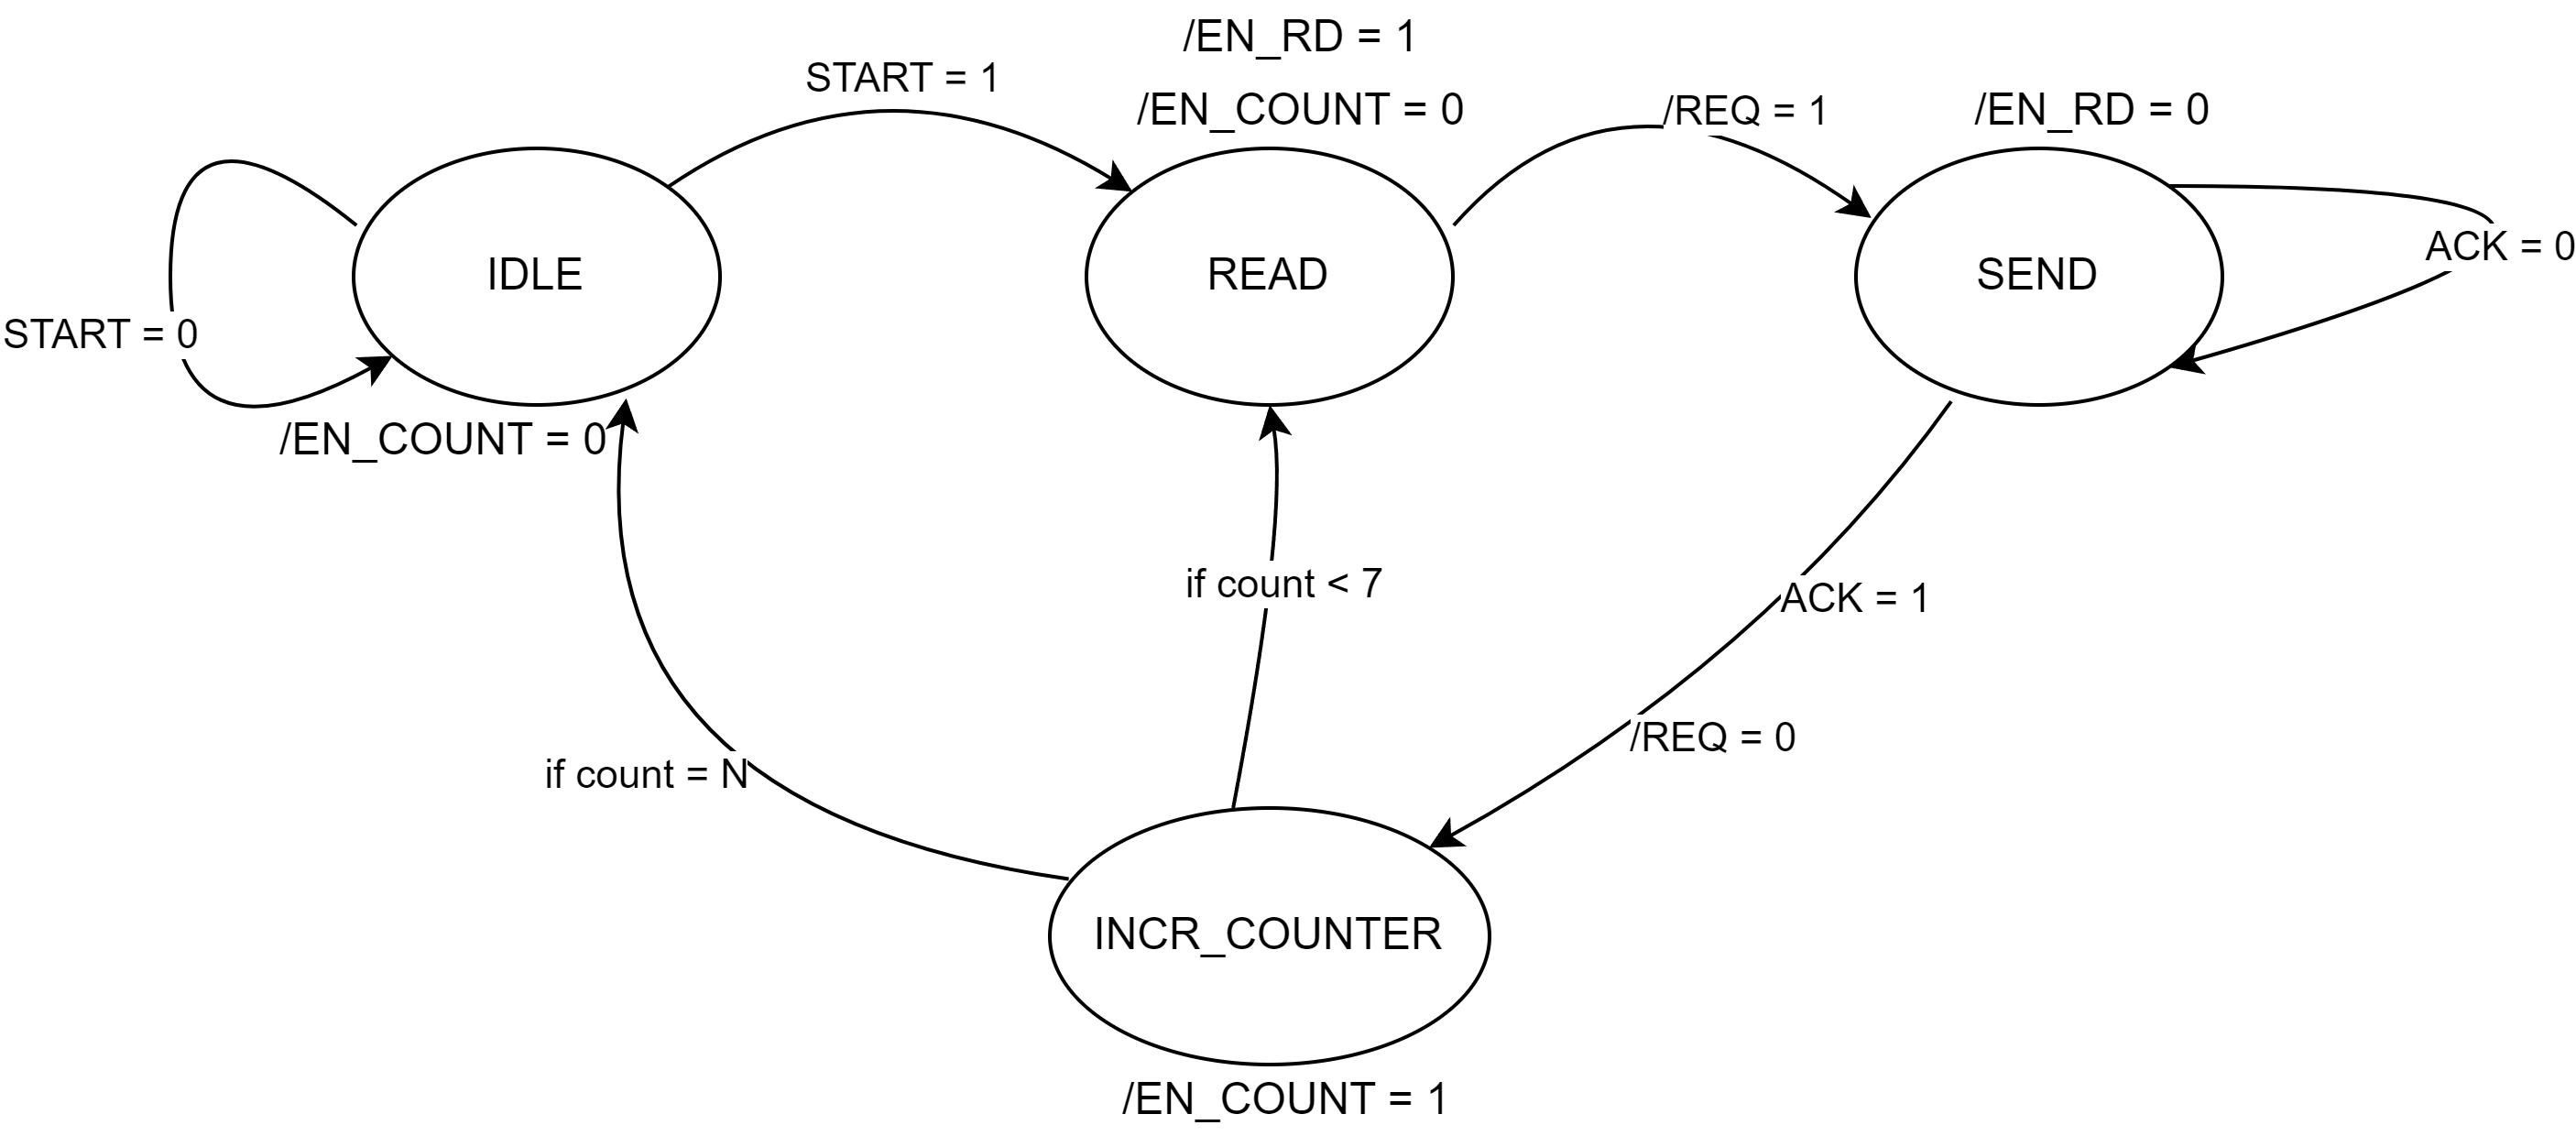
\includegraphics[width=1\textwidth]{img/handshaking/automa_A_handshake}
	\caption{Automa del nodo A}
	\label{test1} 
\end{figure}
\begin{figure}[H]
	\centering
	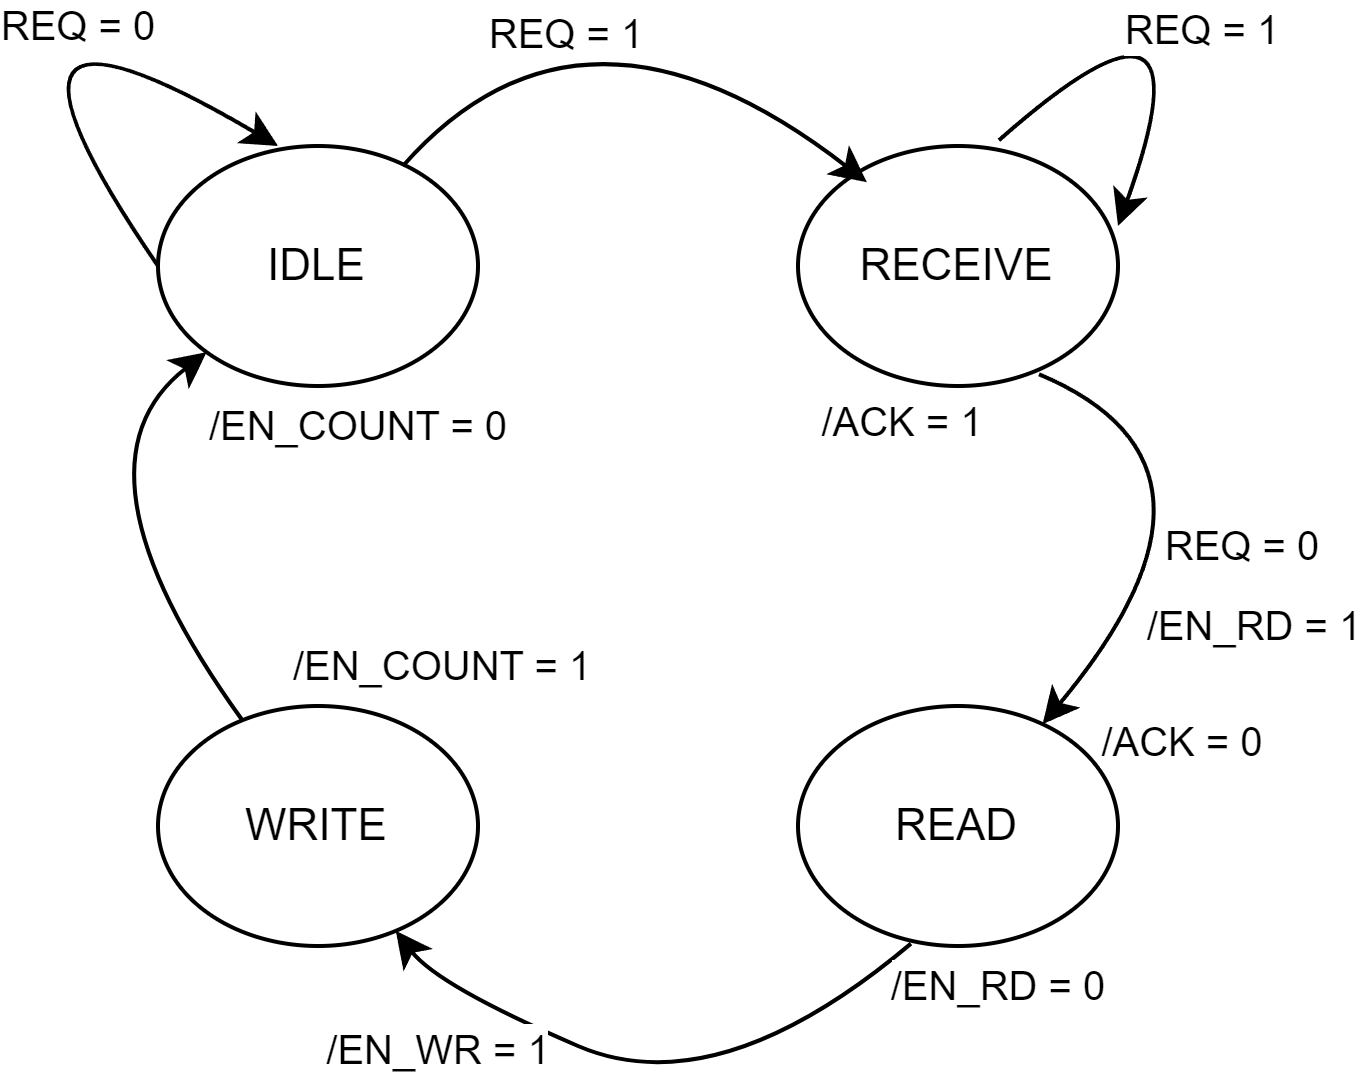
\includegraphics[width=0.8\textwidth]{img/handshaking/automa_B_handshake}
	\caption{Automa del nodo B}
	\label{test1} 
\end{figure}
\subsection{Implementazione}
Per l'implementazione di tale sistema si inizia definendo il nodo A. Come detto, esso si compone di una ROM e un contatore, che insieme costituiscono l'unità operativa, e una unità di controllo per la gestione. Si mostrano i codici relativi all'implementazione del nodo A:
\begin{code}
    \inputminted[frame=lines, framesep=2mm, baselinestretch=1.2, bgcolor=LightGray, fontsize=\footnotesize, linenos]{vhdl}{vhdl_files/handshaking/MEM_A.vhd}
    \caption{MEM\_A.vhdl}
    \label{lbl:ROMC}
\end{code}
\begin{code}
    \inputminted[frame=lines, framesep=2mm, baselinestretch=1.2, bgcolor=LightGray, fontsize=\footnotesize, linenos]{vhdl}{vhdl_files/handshaking/counter.vhd}
    \caption{counter.vhdl}
    \label{lbl:ROMC}
\end{code}
\begin{code}
    \inputminted[frame=lines, framesep=2mm, baselinestretch=1.2, bgcolor=LightGray, fontsize=\footnotesize, linenos]{vhdl}{vhdl_files/handshaking/unita_operativa.vhd}
    \caption{unità operativa di A in vhdl}
    \label{lbl:ROMC}
\end{code}
\begin{code}
    \inputminted[frame=lines, framesep=2mm, baselinestretch=1.2, bgcolor=LightGray, fontsize=\footnotesize, linenos]{vhdl}{vhdl_files/handshaking/UCA.vhd}
    \caption{unità di controllo di A in vhdl}
    \label{lbl:ROMC}
\end{code}
\begin{code}
    \inputminted[frame=lines, framesep=2mm, baselinestretch=1.2, bgcolor=LightGray, fontsize=\footnotesize, linenos]{vhdl}{vhdl_files/handshaking/nodo_A.vhd}
    \caption{nodo A in vhdl}
    \label{lbl:ROMC}
\end{code}
Per quanto riguarda il nodo B, come si vede dallo schema a blocchi, esso è composto da una memoria a cui si accede sia per la lettura che per la scrittura, un contatore e un addizionatore (implementato come Ripple Carry Adder in maniera strutturale a partire da full adder).  Il componente \textit{counter} è comune sia al nodo A che al nodo B, quindi non se ne riporterà nuovamente il codice.  
\begin{code}
    \inputminted[frame=lines, framesep=2mm, baselinestretch=1.2, bgcolor=LightGray, fontsize=\footnotesize, linenos]{vhdl}{vhdl_files/handshaking/MEM_B.vhd}
    \caption{MEM\_B.vhdl}
    \label{lbl:ROMC}
\end{code}
\begin{code}
    \inputminted[frame=lines, framesep=2mm, baselinestretch=1.2, bgcolor=LightGray, fontsize=\footnotesize, linenos]{vhdl}{vhdl_files/handshaking/full_adder.vhd}
    \caption{full\_adder.vhdl}
    \label{lbl:ROMC}
\end{code}
\begin{code}
    \inputminted[frame=lines, framesep=2mm, baselinestretch=1.2, bgcolor=LightGray, fontsize=\footnotesize, linenos]{vhdl}{vhdl_files/handshaking/RCA.vhd}
    \caption{Ripple Carry Adder (approccio strutturale) in vhdl}
    \label{lbl:ROMC}
\end{code}
Tali componenti insieme vanno a costituire l'unità operativa.
\begin{code}
    \inputminted[frame=lines, framesep=2mm, baselinestretch=1.2, bgcolor=LightGray, fontsize=\footnotesize, linenos]{vhdl}{vhdl_files/handshaking/unita_operativa_B.vhd}
    \caption{unità operativa di B in vhdl}
    \label{lbl:ROMC}
\end{code}
Il nodo B è caratterizzato da una sua unità di controllo:
\begin{code}
    \inputminted[frame=lines, framesep=2mm, baselinestretch=1.2, bgcolor=LightGray, fontsize=\footnotesize, linenos]{vhdl}{vhdl_files/handshaking/UCB.vhd}
    \caption{unità di controllo di B in vhdl}
    \label{lbl:ROMC}
\end{code}
Unità operativa e di controllo costituiscono il nodo nel suo complesso.
\begin{code}
    \inputminted[frame=lines, framesep=2mm, baselinestretch=1.2, bgcolor=LightGray, fontsize=\footnotesize, linenos]{vhdl}{vhdl_files/handshaking/nodo_B.vhd}
    \caption{nodo B in vhdl}
    \label{lbl:ROMC}
\end{code}
Il sistema complessivo, è realizzato collegando opportunamente il nodo A e il nodo B, come mostrato in seguito.
\begin{code}
    \inputminted[frame=lines, framesep=2mm, baselinestretch=1.2, bgcolor=LightGray, fontsize=\footnotesize, linenos]{vhdl}{vhdl_files/handshaking/AplusB.vhd}
    \caption{Sistema complessivo (A più B) in vhdl}
    \label{lbl:ROMC}
\end{code}
Il codice commentato nelle implementazioni mostrate è stato utilizzato ed è utilizzabile in fase di debugging, per verificare che l'handshaking funzioni correttamente, e che tutte le stringhe inviate siano ricevute, sommate e memorizzate in modo coerente.
\subsection{Simulazione}
Per la simulazione è necessario utilizzare un testbench.
\begin{code}
    \inputminted[frame=lines, framesep=2mm, baselinestretch=1.2, bgcolor=LightGray, fontsize=\footnotesize, linenos]{vhdl}{vhdl_files/handshaking/testbench.vhd}
    \caption{testbench}
    \label{lbl:ROMC}
\end{code}
Eseguendo la simulazione sull'ambiente di sviluppo Vivado si ottiene la seguente forma d'onda:
\begin{figure}[H]
	\centering
	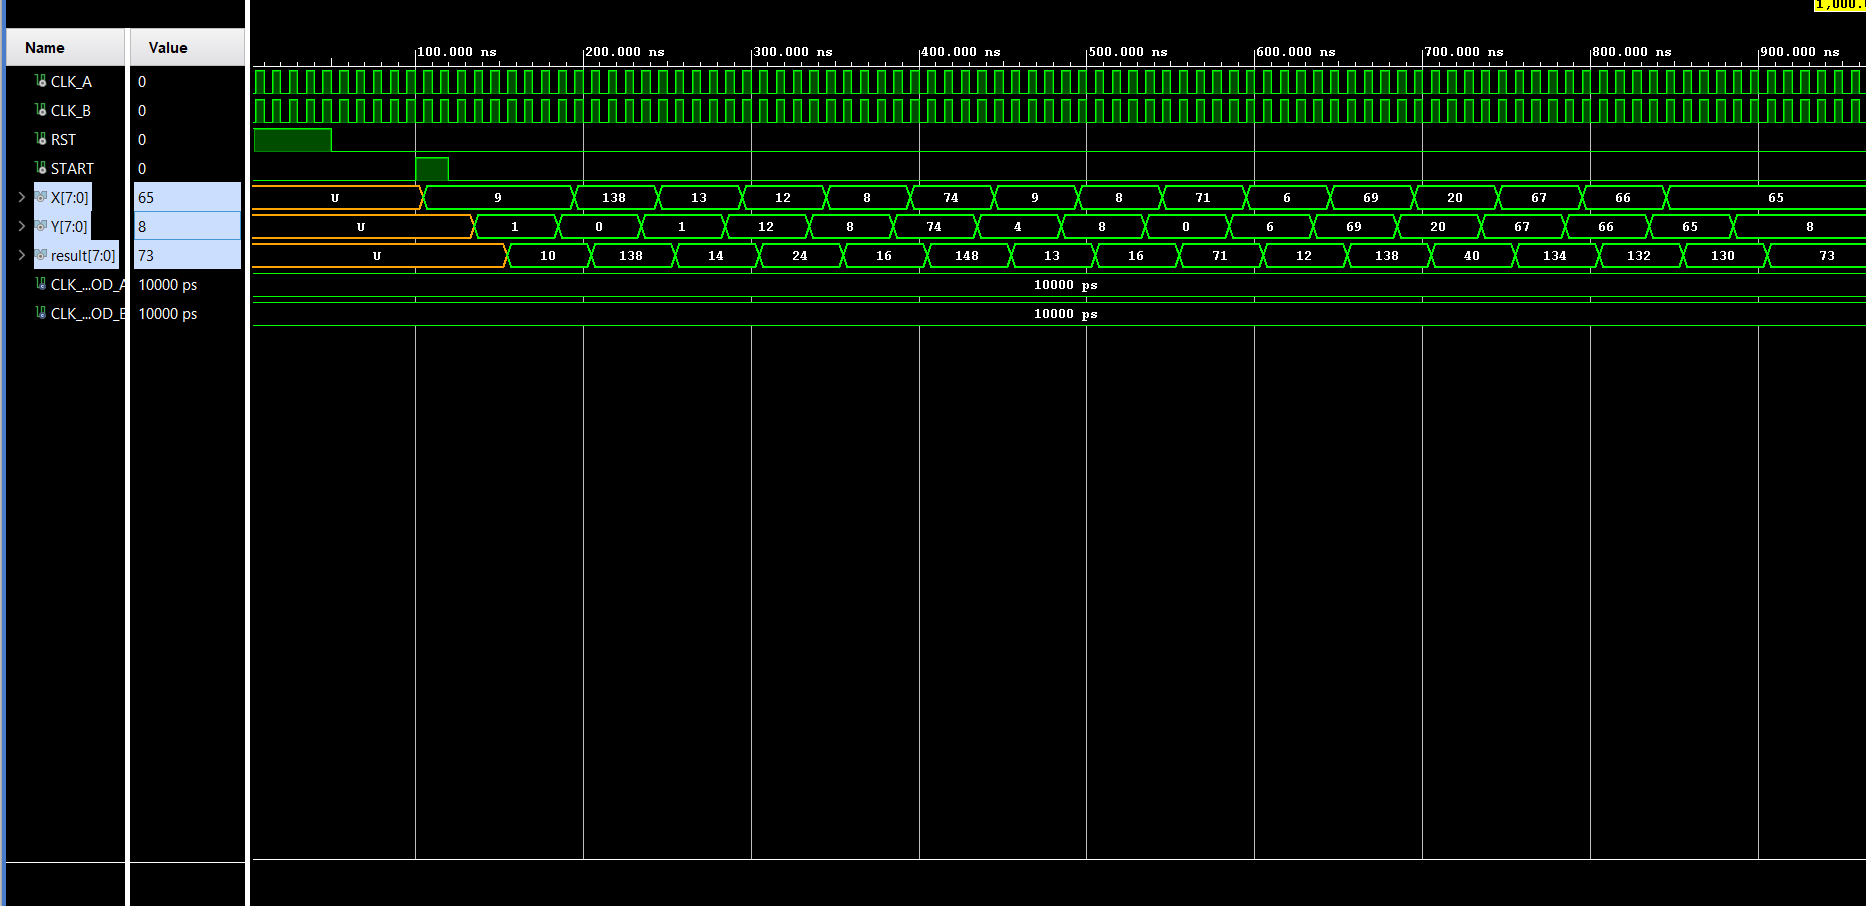
\includegraphics[width=1\textwidth]{img/handshaking/waveform_handshaking}
	\caption{Waveform del sistema}
	\label{test1} 
\end{figure}
Per la conferma del risultato si analizzano le prime locazioni delle memorie di A e B. Si inizia dalla locazione '0':\\
$X(0) = 00001001 $ che in decimale corrisponde a 9;\\
$Y(0) = 00000001$ che in decimale corrisponde a 1;\\
$X(0) + Y(0) = 9 + 1 = 10$.\\
In locazione '1':
$X(0) = 10001010 $ che in decimale corrisponde a 138;\\
$Y(0) = 00000000$ che in decimale corrisponde a 0;\\
$X(0) + Y(0) = 138 + 0 = 138$.\\
In locazione '2':
$X(0) = 00001101 $ che in decimale corrisponde a 13;\\
$Y(0) = 00000001$ che in decimale corrisponde a 1;\\
$X(0) + Y(0) = 13 + 1 = 14$.\\
I risultati possono essere considerati coerenti.